%THIS IS AN EXAMPLE OF HOW YOU MIGHT INTRODUCE A CHAPTER WHICH HAS ALREADY BEEN PUBLISHED.
\cleartoevenpage
\pagestyle{empty}	%Use this to suppress the header from the preceding chapter.

\noindent
The following published manuscript has been incorporated as Chapter~\ref{Chap:3}.

\noindent
\textbf{Wilkinson, Ross D.}, Glen A. Lichtwark, and Andrew G. Cresswell. 2020. The Mechanics of Seated and Nonseated Cycling at Very-High-Power Output: A Joint-Level Analysis. \textit{Medicine $\&$ Science in Sports $\&$ Exercise} 52(7): 1584-94. doi: 10.1249/MSS.0000000000002285

\begin{table}[h]
	\begin{center}
	\begin{tabular}{|c|l|l|}
		\hline
		Contributor & Statement of contribution & $\%$ \\
		\hline
		\textbf{Wilkinson, R.D.} & writing of text & 80\\
        & study design and concept & 20 \\
		& data collection & 90\\
        & data analysis & 90\\
		& statistical analysis & 90 \\
		& preparation of figures & 80 \\
		& revision of written work & 40 \\
		& supervision, guidance & 0 \\
		\hline
		Lichtwark, G.A. & writing of text & 10\\
        & study design and concept & 40 \\
		& data collection & 5 \\
        & data analysis & 5 \\
		& statistical analysis & 5 \\
		& preparation of figures & 10 \\
		& revision of written work & 30 \\
		& supervision, guidance & 50 \\
		\hline
		Cresswell, A.G. & writing of text & 10\\
        & study design and concept & 40 \\
		& data collection & 5 \\
        & data analysis & 5 \\
		& statistical analysis & 5 \\
		& preparation of figures & 10 \\
		& revision of written work & 30 \\
		& supervision, guidance & 50 \\
		\hline
	\end{tabular}
	\end{center}
\end{table}

%-------------------------------------------------------------------------------------------------------%
%-------------------------------------------------------------------------------------------------------%
%-------------------------------------------------------------------------------------------------------%
%-------------------------------------------------------------------------------------------------------%
%-------------------------------------------------------------------------------------------------------%
%-------------------------------------------------------------------------------------------------------%
%This is an internal chapter of the thesis.
%If you have a long title, you can supply an abbreviated version to print in the Table of Contents using the optional argument to the \chapter command.
\chapter[The Mechanics of Seated and Non-Seated Cycling at Very-High-Power Output: A Joint-Level Analysis.]{The Mechanics of Seated and Non-Seated Cycling at Very-High-Power Output: A Joint-Level Analysis.}
\label{Chap:3}	%CREATE YOUR OWN LABEL.
\pagestyle{headings}
%If you are presenting work which has been previously published, acknowledge this here.
%-------------------------------------------------------------------------------------------------------%
%-------------------------------------------------------------------------------------------------------%
%-------------------------------------------------------------------------------------------------------%
\section{Abstract}
Cyclists frequently use a non-seated posture when accelerating, climbing steep hills, and sprinting; yet, the biomechanical difference between seated and non-seated cycling remains unclear. \textbf{Purpose:} To test the effects of posture (seated and non-seated) and cadence (70 rpm and 120 rpm) on joint power contributions, effective mechanical advantage, and muscle activation within the leg during very-high-power output cycling. \textbf{Methods:} Fifteen male participants rode on an instrumented ergometer at $50\%$ of their individualised maximal instantaneous power output ($10.7\pm2.0$ W$\cdot$kg$^{-1}$; above the reported threshold for seated to non-seated transition) in different postures (seated and non-seated) and at different cadences (70 rpm and 120 rpm), whilst lower-limb muscle activity, full-body motion capture and crank radial and tangential forces were recorded. A scaled, full-body model was used to solve inverse kinematics and inverse dynamics to determine joint displacements and net joint moments. Statistical comparisons were made using a two-way, repeated-measures analysis of variance (posture $\times$ cadence). \textbf{Results:} There were significant main effects of posture and cadence on joint power contributions. A key finding was that the non-seated posture increased negative power at the knee, with an associated significant decrease of net power at the knee. The contribution of knee power decreased by $15\%$ at both 70 and 120 rpm ($\sim0.8$ W$\cdot$kg$^{-1}$) when non-seated compared to seated. Subsequently, hip power and ankle power contributions were significantly higher when non-seated compared to seated at both cadences. In both postures, knee power was $9\%$ lower at 120 rpm compared to 70 rpm ($\sim0.4$ W$\cdot$kg$^{-1}$). \textbf{Conclusion:} These results evidenced that the non-seated posture significantly decreases net mechanical power requirements at the knee when cycling at high power outputs, however the effect is cadence dependent.

\section{Introduction}
Cyclists often transition from a seated to a non-seated posture during short, intensive bouts of climbing, accelerating and sprinting \autocite{Costes2015}. An increased understanding of the biomechanical differences between the seated and non-seated posture has practical importance for cycling performance and equipment design \autocite{Hansen2008}, as well as injury prevention and rehabilitation \autocite{Stone1993}. The non-seated posture is typified by cyclists raising their pelvis off the saddle, which results in a more extended hip and knee angles, an alteration of the direction of the resultant crank force \autocite{Caldwell1998} and an effective use of body mass to generate positive power at the crank during the downstroke \autocite{Stone1995}. Although it is known that the non-seated posture is more effective than the seated posture for peak maximal power production \autocite{Millet2002,ReiserII2002} cyclists often transition off the saddle well before their limit of power production is reached \autocite{Costes2015,Poirier2007}. For example, using an incremental testing protocol within a laboratory setting it was determined that non-cyclists spontaneously transitioned to a non-seated posture at $568\pm93$ watts ($7.9\pm1.4$ W$\cdot$kg$^{-1}$) when pedalling at a cadence of $90$ rpm \autocite{Costes2015}, well below the 6-sec maximal power production measured in a similar untrained population of $813\pm137$ watts ($12.4\pm1.3$ W$\cdot$kg$^{-1}$) \autocite{Vandewalle1987}. 

Field testing \autocite{Hansen2008} has shown that competitive cyclists can increase their time to exhaustion during uphill cycling by using the non-seated posture when the required power output is at or above $419\pm30$ watts ($5.6\pm0.4$ W$\cdot$kg$^{-1}$). In the same study, it was shown that preferred cadence decreased from $92\pm2$ rpm when seated to $74\pm3$ rpm when non-seated. This preference for a lower cadence when non-seated implies that cyclists favour generating power at the crank by increasing crank torque and reducing crank angular velocity. Thus, if we assume the range of motion at each lower-limb joint to be similar between postures, one of the possible benefits of the transition could be that it alters the conditions under which the muscles perform work or allows cyclists to redistribute the work requirements to different muscles. Currently no methods exist to directly measure this redistribution at a muscular level, however the integration of inverse dynamics and electromyography (EMG) may provide indirect evidence of these changes.

Joint-level analyses of seated cycling have shown that the distribution of total lower limb power among the hip, knee and ankle is sensitive to the torque and angular velocity demands \autocite{Elmer2011,Lieber1993}. For example, Elmer et al. \autocite{Elmer2011} reported that as net crank power increased from $250$ to $850$ watts at a constant cadence of $90$ rpm (i.e. increasing torque demand), the contribution of knee extension power decreased, whereas the contribution of knee flexion power increased. A similar analysis of seated maximal sprint cycling by McDaniel et al. \autocite{McDaniel2014} found that as cadence increased from $60$ rpm to $180$ rpm the contribution of hip extension power and knee flexion power increased, while the contribution of knee extension power did not change. These findings provide an indication of how joint power is likely to be redistributed in response to changes in power output and cadence, however it is not known whether a similar redistribution of joint power will occur when non-seated, or if the initial distribution of total lower limb power is similar to when seated.

EMG analyses have provided insight into the sources of power generation during non-seated cycling \autocite{Li1998,Turpin2016}, however fundamental mechanical differences between the seated and non-seated posture remain unresolved. These gaps exist as previous research has primarily focused on either performance \autocite{ReiserII2002,Hansen2008} or physiological economy differences \autocite{Millet2002,Tanaka1996,Harnish2007} between the two postures. Thus, biomechanical assessments of the non-seated posture remain incomplete and allow only speculation of the underlying mechanical interaction of muscles and body segments. It seems likely that the kinematic differences between the seated and non-seated posture; notably the anterior shift in the rider's CoM and more extended hip and knee position, will impact the pattern of power production and absorption within the lower limb, especially at the knee. Yet to date, no study has determined whether the distribution of lower limb power among the hip, knee and ankle differs between the seated and non-seated postures.

The present study was designed to compare the distribution of joint powers between seated and non-seated postures during high power output cycling at two different cadences. Effective mechanical advantage and muscle activity in the lower limb was also compared between the postures under these same cadence and power conditions. It was predicted that at a constant external power output, the net contribution of knee power would be lower in the non-seated posture compared to seated at each cadence and that the redistribution of this power would be cadence dependent. It was also predicted that a decrease in both the peak knee extension moment and net knee power in the non-seated posture would be associated with improved effective mechanical advantage at the knee compared to when seated.

\section{Methods}
\subsubsection{Participants}
Fifteen active and healthy males (age $30\pm8$ years, height $1.79\pm0.05$ m; mass $74\pm9$ kg) volunteered to participate in this study. The athletic background of the participant group was varied. Eight of the participants were cyclists who competed weekly at club level, while the remainder regularly engaged in a variety of competitive or recreational sports. All participants gave their written informed consent prior to participating in this study according to the procedures approved by the Human Ethics Committee of The University of Queensland and in accordance with the general principles expressed in the Declaration of Helsinki.

\subsection{Experimental protocol}
Participants performed five 3-s all-out seated sprints to determine their peak instantaneous maximal power ($P_{max.i}$) followed by four sub-maximal trials at $50\%$ of their individual $P_{max.i}$ under different combinations of posture (seated or non-seated) and cadence ($70$ rpm or $120$ rpm); outlined below.

\subsubsection{Ergometer setup}
Once the participants were deemed fit for testing, their body mass, height, inside leg length, torso length, arm length and shoe size were measured. These measures were then used to fit the participants to the cycling ergometer, which was used for all trials (Excalibur Sport, Lode BV, Groningen, The Netherlands). Seat tube angle was standardised to $73^\circ$ with respect to horizontal and knee angle was standardised to $150^\circ$ of extension when the right pedal was at its lowest position. This angle was measured using a goniometer with the participant in a static, seated posture on the ergometer. Knee angle was determined from the bisection of two lines connecting markers placed on the greater trochanter, lateral femoral condyle and lateral malleolus. The saddle height and fore-aft position of the saddle were incrementally adjusted until the desired combination of knee angle and seat tube angle were achieved. Torso angle was standardised to $70^\circ$, with arms slightly bent at the elbow and hands placed in the drops of the handlebar. Torso angle was defined with respect to horizontal by the line connecting markers placed on the acromion process and greater trochanter. Some minor adjustments to this fitting were allowed based on participant preference. Crank length was constant at $175$ mm. Participants wore a standardised model of cleated cycling shoe (SH-R070, Shimano, Osaka, Japan) that clipped into the pedals (SH-R540, Shimano, Osaka, Japan). 

\subsubsection{Maximal power output test ($P_{max.i}$)}
Participants began with a 5-min cycling warm-up at $100$ W at their preferred cadence. Participants then performed five maximal sprints of 3-s duration in a seated posture to determine their individual $P_{max.i}$. The ergometer was set to ``Linear'' mode, which ensured that power was coupled to cadence. It was expected that participants would achieve $P_{max.i}$ at a cadence of approximately $120$ rpm \autocite{Gardner2007,Dorel2005,Dorel2018a}. Thus, the linear resistance was increased or decreased for each subsequent trial based on whether the participant achieved a peak cadence above or below $120$ rpm. $P_{max.i}$ was successfully determined within five trials for all participants and was calculated as the highest ``instantaneous'' power that occurred during a crank cycle. Participants were given 3 min of rest between trials to reduce any potential fatigue effects.

\subsubsection{Sub-maximal trials}
A 20-min period of rest was given after the $P_{max.i}$ test before commencing the four sub-maximal trials. The constant power output and cadence ($70$ rpm or $120$ rpm) conditions for the sub-maximal trials were chosen with the intention to create two scenarios where cyclists would prefer to ride in a non-seated position. This assumption was based on the reported seated to non-seated transition power at $90$ rpm \autocite{Costes2015}, and that this transition power is dependent upon the amount of torque required per crank cycle. Thus, the power output had to be high enough for riders to still want to ride off the saddle at $120$ rpm, while low enough that it was still achievable at $70$ rpm in both postures. Pilot testing revealed that $50\%$ of individual $P_{max.i}$ measured at approximately $120$ rpm would be appropriate for this purpose. The two cadence conditions of $70$ rpm and $120$ rpm were chosen primarily to provide a contrast in the amount of torque required per cycle, however they also happen to be approximately equal to preferred cadences used during climbing \autocite{Lucia2001} and sprinting \autocite{Gardner2007}, respectively. It should be noted that the selected power output and cadences were not intended to simulate the exact conditions of sprinting or climbing. Participants performed the combinations of posture and cadence in a randomised order and were required to maintain the target cadence and power output for a minimum period of 10-sec. The ergometer was set to ``Hyperbolic'' mode, which ensures that the power output remains constant independent of cadence, thus riders were required to maintain the specific set cadences using feedback from the visual display on the ergometer. To test for the presence of any exercise-induced fatigue, an additional 3-s maximal sprint was performed following the sub-maximal trials. Inclusion required the participants to be able to match ($\pm5\%$) their previously tested $P_{max.i}$ in this additional trial. Kinematics, kinetics and EMG were recorded during the sub-maximal trials.

\subsection{Data collection}
All analogue signals were acquired using a 16-bit analogue-to-digital (A/D) conversion board (USB-2533, Measurement Computing Corporation, Norton, MA) using Qualisys Track Manager software (Qualisys AB, Gothenburg, Sweden).

\subsubsection{Motion capture}
An eight camera, opto-electronic motion capture system (Oqus, Qualisys, AB, Sweden) was used to measure the three-dimensional (3D) position of 45 passive reflective markers at 200 Hz. Markers were secured using double-sided tape over the suprasternal notch, vertebrae C7, sacrum, and bilaterally over the acromion processes, lateral epicondyles of the humerus, styloid processes of the radius, iliac crests, anterior superior iliac spines, posterior superior iliac spines, greater trochanters, medial and lateral condyles of the femur, medial and lateral malleoli, calcanei, heads of the 1st and 5th metatarsals and the 2nd distal phalanxes (marker placements are shown in Figure \ref{fig:m1f1}). Lightweight rigid clusters of four markers were also secured bilaterally to the lateral mid-thighs and lateral mid-shanks using double-sided tape and self-adhesive bandage. Prior to the sub-maximal trials, marker positions were captured with the participant standing in a standard anatomical posture. This static trial was later used for scaling purposes during data processing. The heading (yaw) angle of the ergometer was determined relative to the motion capture global coordinate system by placing two passive reflective markers on the rear support legs of the ergometer. These markers were used to establish a local coordinate system for the ergometer, which accounted for any discrepancy with the global coordinate system between trials.

\subsubsection{Crank angle and forces}
Tangential and radial forces to the left and right crank, and crank angle were recorded at 100 Hz using pre-calibrated, wireless, instrumented cranks (Axis, SWIFT Performance, Brisbane, Australia). Digital signals were transmitted wirelessly to a base receiver and then converted to an analogue signal through the A/D Board. The digital sampling frequencies of the crank ($100$ Hz) and EMG ($2$ kHz) were matched to the motion capture ($200$ Hz) sampling frequency using the internal sampling factor within the Qualisys Track Manager software. A multi-axis, dynamic calibration of each crank was performed in-house by the fabricating company (Swift Performance, Australia). In addition and prior to testing, voltage offsets for tangential and radial force signals were determined by hanging a known mass of $2.5$ kg from each pedal spindle with the cranks in a horizontal and vertical position, which allowed any discrepancy in the offset to be removed post-processing. The crank angle signal was zeroed with the right crank at top dead centre (TDC).

\subsubsection{Electromyography}
Surface EMG signals of gluteus maximus (GMax), rectus femoris (RF), long head of biceps femoris (BF), vastus lateralis (VL), gastrocnemius medialis (MG) and soleus (SOL) were recorded wirelessly from the right leg at $2$ kHz (Myon AG, Baar, Switzerland). Before electrode application, the skin at each recording site was shaved, abraded and cleaned to reduce impedance. Bipolar electrodes (Ag/AgCl, Covidien, Mansfield, MA) were then placed according to SENIAM recommendations, except for SOL which was placed medial to the muscle belly and parallel to its fibre pennation angle. Each signal was then checked for clarity and strength during an attempted isolated contraction. All cables and electrodes were then secured to the skin using a combination of adhesive tape and self-adhesive bandage to minimise movement artefact.

\subsection{Data analysis}
\subsubsection{Joint power}
3-D motion capture marker trajectories were labelled and exported with all analogue data (EMG, crank force and angle) to MATLAB (R2017a, Mathworks Inc., USA) where they were processed using custom scripts. Crank force signals and marker trajectories were zero-lag low-pass filtered at $12$ Hz using a digital second order Butterworth filter \autocite{Kristianslund2012}. The position (angle) signal collected for the right crank was used to create an anti-phase signal which was used as the angle of the left crank. These angle signals were converted to the global coordinate system and then used to convert the respective crank forces (tangential and radial) into their horizontal and vertical components with respect to the same global coordinate system. These force components, along with the marker trajectories, were then rotated into the ergometer coordinate system using 2-D and 3-D rotation matrices, respectively. The origin of the resultant force was determined by creating a virtual marker at the centre of the cleat attachment. This approximation was determined using the crank angle, three-dimensional shoe orientation and shoe size and then verified against a second approximation using the bottom bracket position, crank length, crank angle and pedal spindle length. 

Inverse kinematics and inverse dynamics were calculated using OpenSim software \autocite{Delp2007}. First, a previously developed generic full-body musculoskeletal model \autocite{Rajagopal2016}, was scaled to each participant's anthropometry. Segment length of the upper limbs, torso and lower limbs were scaled in all three axes using the distance between nominated marker pairs. Scaling factors were calculated by comparing these distances to that of the generic model. The mass of the participant was then used in combination with these scaling factors to distribute segment masses. This scaled model as well as the kinematic and kinetic data collected during the sub-maximal trials were used to run inverse kinematics and inverse dynamics via the Application Programming Interface between OpenSim and MATLAB. The inverse kinematics tool within OpenSim calculates joint angles at each time step by using a weighted least squares fit to minimise errors between the experimental markers and model markers. These results are then combined with external loads applied to the model, in this case reaction forces at the left and right crank, to determine the net joint moment at the ankle, knee and hip joints. Joint power was calculated as the dot product of the net joint moment and joint angular velocity. Flexor moments and flexion velocity were defined as positive. Joint powers were then summed and integrated to calculate joint work. Net joint work was the integral of all joint power values over a complete crank cycle starting and finishing at TDC. Total positive and negative work were the integral of all positive and negative powers, respectively, over the same range \autocite{Winter2009}. Individual joint work contributions to total work were calculated by dividing individual net joint work by the summed net joint work of the hip, knee and ankle. Data from the sub-maximal trials were averaged across five cycles of the right crank where the participant was able to match the target power ($\pm5\%$) and cadence ($\pm5\%$). If the participant failed to simultaneously match the target power and cadence the data was excluded from the analysis. The minimum number of crank cycles used to average participant data in this study was two.

\subsubsection{Muscle activity}
DC offset was removed from the raw EMG signal for each muscle prior to band-pass filtering between $20-400$ Hz.  The signals were then rectified and low pass filtered at $15$ Hz using a fourth order zero-lag digital Butterworth filter. The resulting EMG signals were interpolated to $361$ data points per cycle to enable a mean signal to be calculated over $5$ crank cycles. The mean signals were then normalised to the peak EMG RMS value from the trial in which the participant achieved $P_{max.i}$. Due to movement artefact a number of trials for specific recording sites were discarded. Results for GMax, RF and VL were averaged across $14$ participants, MG and SOL were averaged across $12$ participants and BF was averaged across $10$ participants.

\subsubsection{Effective Mechanical Advantage}
As defined by Biewener \autocite{Biewener1989}, ``effective mechanical advantage (EMA) is the ratio of the extensor muscle moment arm ($r$) to the moment arm of the ground reaction force ($R$) acting about the joint.'' In cycling the reaction force on the crank takes the place of the ground reaction force for this ratio. Hence, closer alignment of the joint centre of rotation to the crank reaction force vector will increase a muscle group's EMA. Extensor muscle moment arms ($r$) of the right hip, knee and ankle were calculated within OpenSim software using the moment arms of gluteus maximus as the hip extensor moment arm, vastus lateralis for the knee and soleus for the ankle. In each condition, EMA of hip extensors, knee extensors and ankle plantar flexors were calculated at the time of the peak resultant crank force.

\subsection{Statistical analyses}
A two-way, repeated-measures ANOVA was performed to test for main effects of posture and cadence and interaction effects (posture$\times$cadence) on relative joint power, EMA and mean EMG RMS. The alpha level for main and interaction effects was set at $0.037$ prior to statistical analysis. This alpha level was based on a desired false positive risk of $<5\%$, a prior probability for a real effect of $0.5$, sample size of fifteen and an estimated effect size of $1$ \autocite{FPRcalc}. As per recommendations \autocite{Bakeman2005,Lakens2013}, the F-value ($F$), p-value ($\rho$), and generalised eta squared ($\eta^2_G$) are provided for main and interaction effects. The $\eta^2_G$ for each variable was assessed against the benchmarks of trivial ($<0.0099$), small ($0.0099-0.0588$), moderate ($0.0588-0.1379$), and large effect ($>0.1379$) \autocite{Lakens2013}. All values are reported as mean $\pm$ SD.

\begin{figure}[htbp]
    \centering
    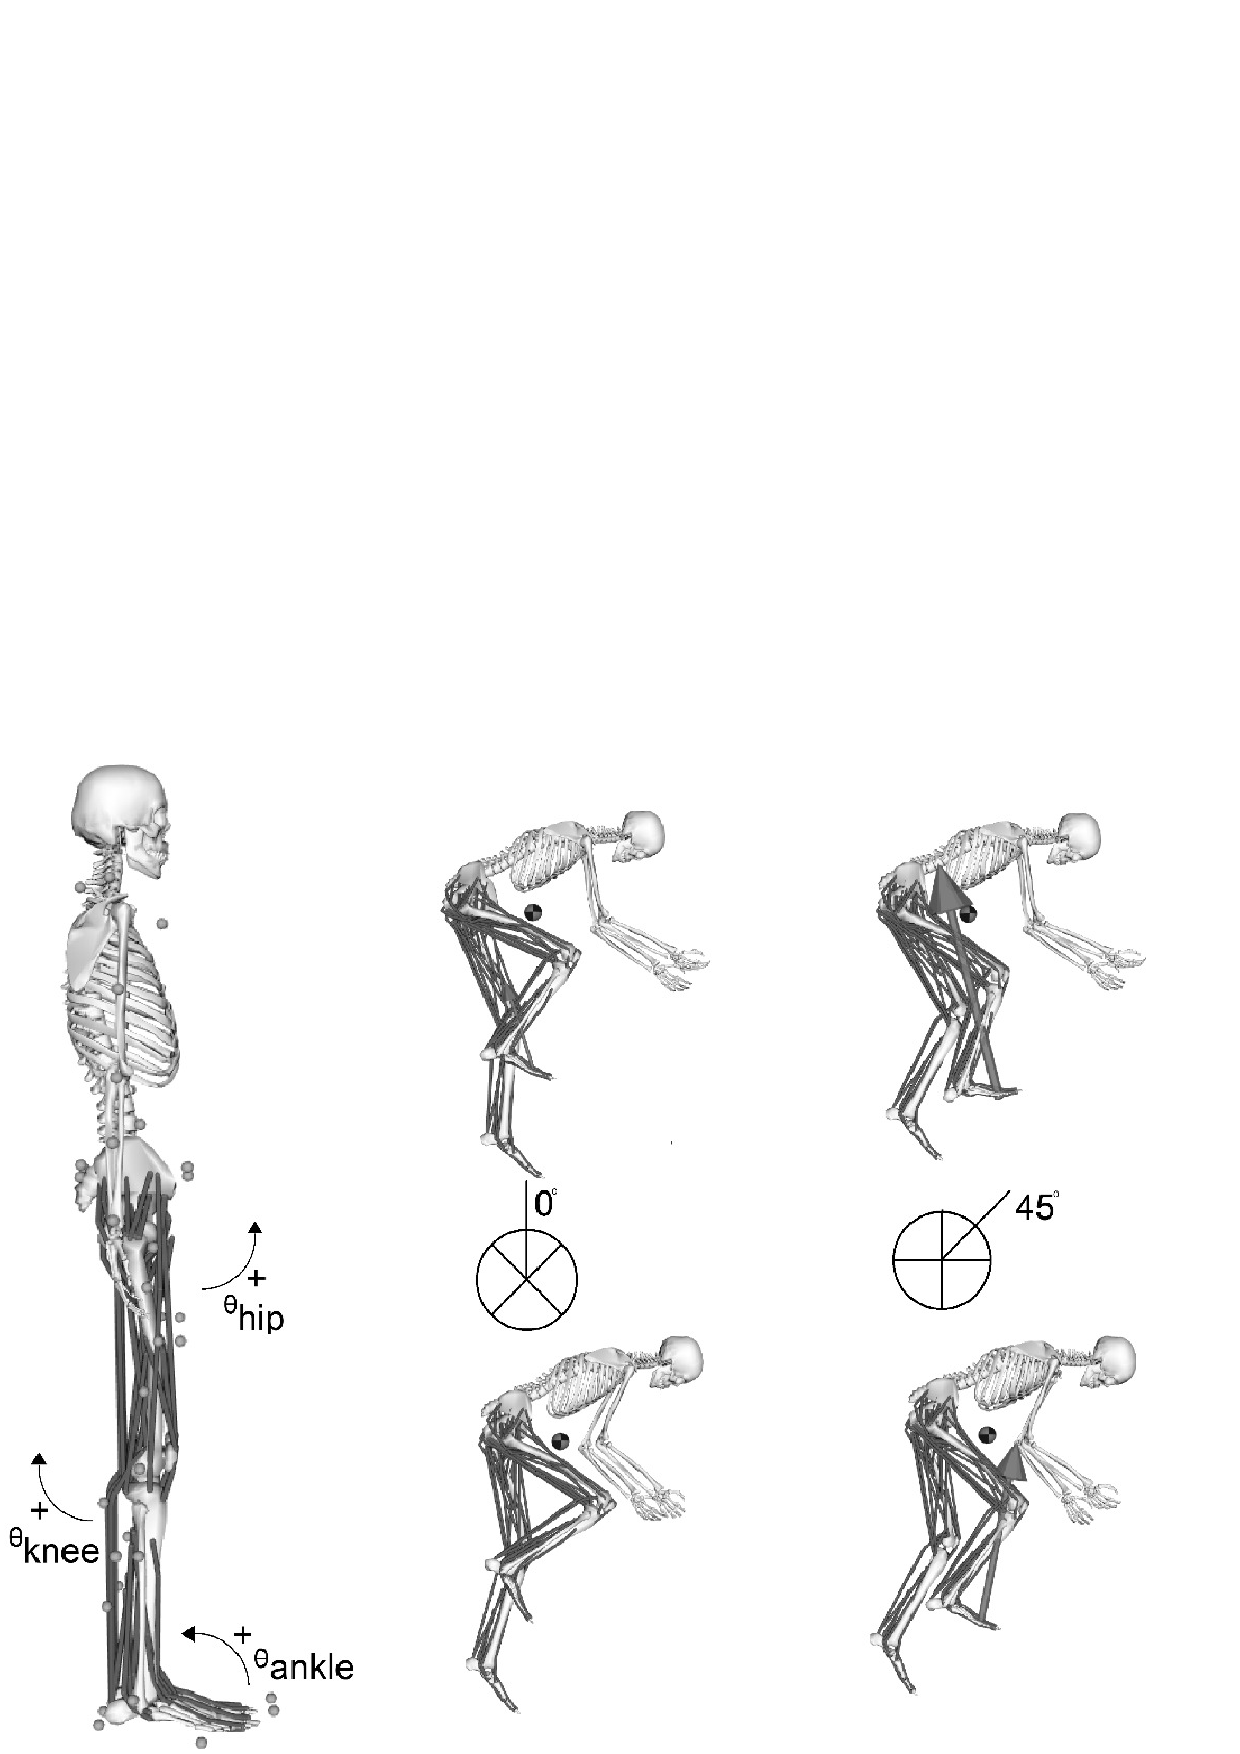
\includegraphics[width=\textwidth]{Study1/Figure1.png}
    \caption[Switching to a non-seated posture shifts peak force production to later in the crank cycle]{\textbf{Switching to a non-seated posture shifts peak force production to later in the crank cycle.} Sagittal-plane images of a representative participant during a static trial (left) showing the definition of hip, knee and ankle joint angles and marker positions; and during seated and non-seated cycling at $70$ rpm for five selected crank positions during the downstroke ($0^\circ$, $45^\circ$, $90^\circ$, $135^\circ$, $180^\circ$). Arrows represent the magnitude and direction of the resultant crank reaction force vector. Grey and black circle represents the participant's CoM position. N.B. The clockwise shift in force production when non-seated compared to seated.}
    \label{fig:m1f1}
\end{figure}
\FloatBarrier

\section{Results}
The mean $P_{max.i}$ across the participant group was $1605\pm368$ W ($21.5\pm4$ W$\cdot$kg$^{-1}$), giving a mean power output of $10.7\pm2.0$ W$\cdot$kg$^{-1}$ for the sub-maximal trials. We individualised the mean crank power output over a complete crank for the sub-maximal trials ($10.7\pm2.0$ W$\cdot$kg$^{-1}$) as $50\%$ of each participant's $P_{max.i}$ recorded during the maximal power output test. Thus, the power output for the sub-maximal trials was $\sim85\%$ of each participant's mean maximal power output ($P_{max.m}$) recorded during the maximal power output test (See Table \ref{tab:m1t1}). Furthermore, due to the effect of cadence on maximal power production it is likely that the sub-maximal power output was near maximal during the $70$ rpm conditions. There was good agreement between the target power and cadences, with power and cadences measured at the crank during each sub-maximal trial (See Table \ref{tab:m1t1}). Group mean crank torque, velocity and power curves with respect to crank angle during the $P_{max.i}$ and sub-maximal trials have been provided as supplementary information (See Figure, Appendix \ref{fig:m1sdc1}). There was a clear rightward phase shift in crank resultant force, velocity and power when non-seated compared to seated, as well as a large difference between crank power and lower limb power during the downstroke, as has previously been demonstrated \autocite{Elmer2011}.

Mean power production at the hip, knee and ankle with respect to crank angle are shown in Figure \ref{fig:m1f2}, from which clear effects of posture and cadence can be seen. At $70$ rpm, power curves for all joints are phase shifted to the right when non-seated, however this phase shift is less pronounced at $120$ rpm. In all conditions the crank cycle begins with power being generated predominantly through knee extension. At $70$ rpm, this contribution is much greater in the seated posture, but similar between postures at $120$ rpm. The power generation phase at the knee is followed by an absorption phase, which occurs simultaneously with hip extension and ankle plantar flexion power. During this period the hip contributes significantly more power at $120$ rpm than at $70$ rpm. At $70$ rpm, the ankle begins the crank cycle with a small period of negative plantar flexion power in both postures, after which its positive power steadily increases. Positive power contributions at the hip and knee during the second half of the crank cycle are clearly visible.

All statistics (F-value ($F$), p-value ($\rho$), generalised eta squared ($\eta^2_G$)) relating to the effects of posture and cadence on joint power contributions have been provided in Table \ref{tab:m1t2}. This analysis revealed main effects of posture on net joint power contributions, which resulted in a moderate increase in hip power, a large decrease in knee power and a large increase in ankle power in the non-seated compared to seated posture (Figure \ref{fig:m1f3}A). At both cadences, knee power in the non-seated posture was $15\%$ ($0.8$ W$\cdot$kg$^{-1}$) less than when seated. At $70$ rpm, hip power increased by $10\%$ ($0.55$ W$\cdot$kg$^{-1}$) and ankle power by $5\%$ ($0.26$ W$\cdot$kg$^{-1}$) in the non-seated compared to seated posture. At $120$ rpm, hip power increased by $12\%$ ($0.78$ W$\cdot$kg$^{-1}$) and ankle power by $3\%$ ($0.25$ W$\cdot$kg$^{-1}$) in the non-seated compared to seated posture. Interestingly, net knee power was lower than net hip and ankle power in all conditions. There was also a main effect of cadence on the power contributed at each joint, which resulted in a large increase in hip power, a moderate decrease in knee power, and a large decrease in ankle power when cycling at $120$ rpm compared to $70$ rpm (See Table \ref{tab:m1t2}).

The contribution of each joint to both positive and negative power is shown in Figure \ref{fig:m1f3} (B-D). In all conditions the knee contributed positive power in the first and third quarter of the crank cycle, however, this was offset by large amounts of negative power during the second quarter. There was a $21.5\%$ increase in negative power during knee extension when non-seated ($-0.8$ W$\cdot$kg$^{-1}$) compared to seated ($-0.6$ W$\cdot$kg$^{-1}$) at $70$ rpm and a $22.4\%$ increase in negative power during knee extension when non-seated ($-0.9$ W$\cdot$kg$^{-1}$) compared to seated ($-0.7$ W$\cdot$kg$^{-1}$) at $120$ rpm. Hip flexion power accounted for $24\pm6\%$ ($1.1$ W$\cdot$kg$^{-1}$) of positive hip power when non-seated at $120$ rpm compared to $20\pm9\%$ ($0.8$ W$\cdot$kg$^{-1}$) when seated. When seated at $70$ rpm, knee flexion power accounted for $32\pm8\%$ ($0.6$ W$\cdot$kg$^{-1}$) of positive knee power compared to $27\pm13\%$ ($0.4$ W$\cdot$kg$^{-1}$) when non-seated. At $120$ rpm, knee flexion power accounted for $44\pm11\%$ ($0.8$ W$\cdot$kg$^{-1}$) of positive knee power compared to only $34\pm10\%$ ($0.5$ W$\cdot$kg$^{-1}$) when non-seated.

\begin{figure}[htbp]
    \centering
    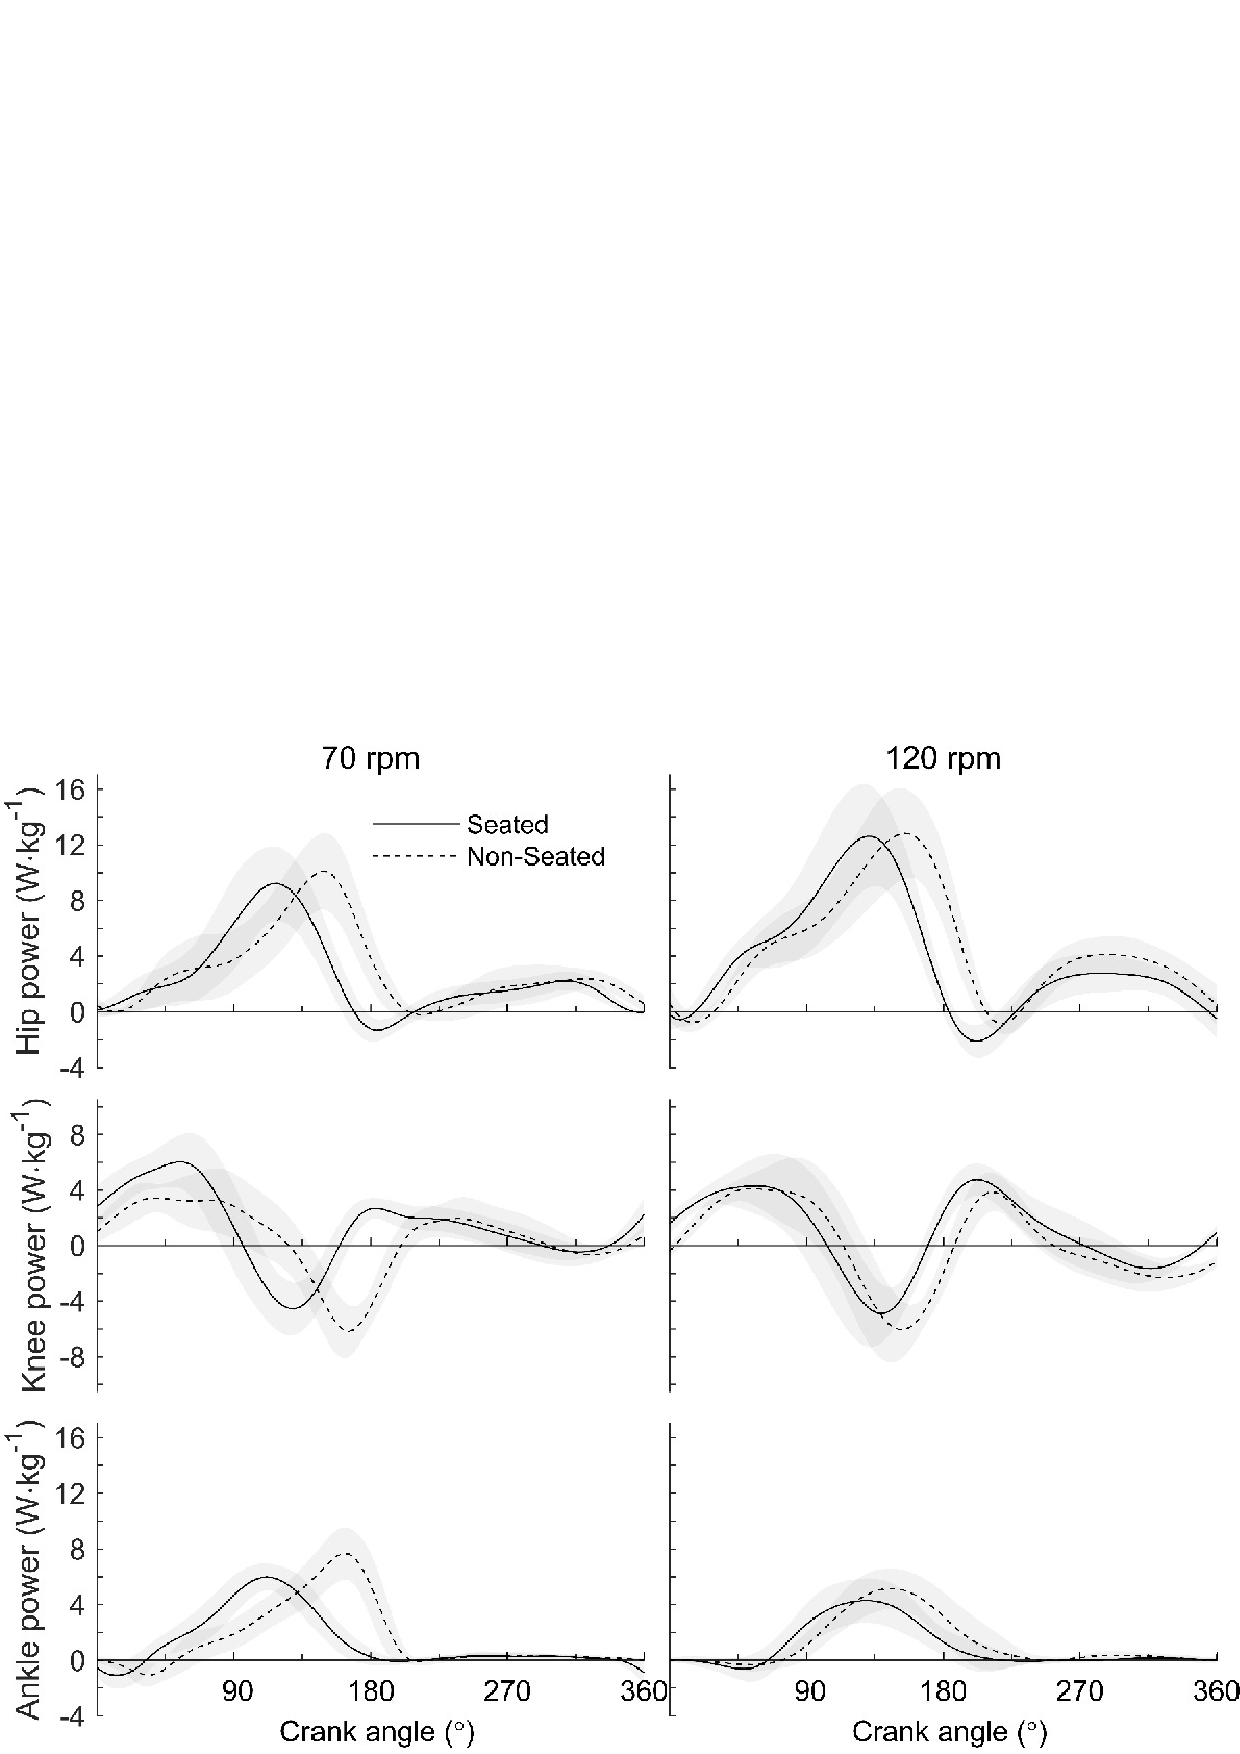
\includegraphics[width=\textwidth]{Study1/Figure2.png}
    \caption[Joint power production occurs later in the crank cycle when in a non-seated posture compared to seated.]{\textbf{Joint power production occurs later in the crank cycle when in a non-seated posture compared to seated.} Comparison of group mean ($\pm$SD; shaded area) hip, knee and ankle power in the right lower limb between the seated (solid lines) and non-seated (dashed lines) posture during high-power output cycling at $70$ rpm and $120$ rpm. N.B. Power curves are visibly phase shifted to the right when non-seated, particularly at $70$ rpm. Knee power curves are characterised by a significant period of negative power during the downstroke.}
    \label{fig:m1f2}
\end{figure}
\FloatBarrier

% \begin{figure}[htbp]
%     \centering
%     \includegraphics[width=\textwidth]{Study1/Table1.png}
%     \caption[There was a significant main effect of posture at the hip, knee, and ankle during high-power output cycling.]{\textbf{There was a significant main effect of posture at the hip, knee, and ankle during high-power output cycling.} Group mean ($\pm$SD) right crank power, right leg power and joint-specific power relative to body mass during seated and non-seated cycling at 70 rpm and 120 rpm.}
%     \label{tab:m1t1}
% \end{figure}

\begin{table}[htbp]
    \centering
    \ra{1.5}
    \begin{tabularx}{\textwidth}{@{}l*{7}{r}@{}}
        \toprule
         & \multicolumn{1}{c}{Sprint} && \multicolumn{2}{c}{70 rpm} && \multicolumn{2}{c}{120 rpm} \\
         \cmidrule{2-2} \cmidrule{4-5} \cmidrule{7-8}
         & \multicolumn{1}{c}{Seated} && \multicolumn{1}{c}{Seated} & \multicolumn{1}{c}{N-S} && \multicolumn{1}{c}{Seated} & \multicolumn{1}{c}{N-S}\\
        \midrule
        Mean cadence (rpm) & $120\pm2$ && $70\pm3$ & $71\pm3$ && $118\pm4$ & $119\pm4$\\
        \hdashline[1pt/3pt]
        Mean tot. crank pwr (W/kg) & $13.5\pm2.5$ && $11.3\pm1.5$ & $11.5\pm1.6$ && $11.2\pm1.6$ & $11.4\pm1.5$\\
        % \hdashline[1pt/3pt]
        \hspace{0.5cm} as a \% of P_{max.i} & $63\pm4$ && $53\pm5$ & $54\pm6$ && $53\pm5$ & $54\pm5$\\
        \hdashline[1pt/3pt]
        Max. inst. crank pwr (W/kg) & $21.5\pm4.0$ && $15.7\pm1.3$ & $18.0\pm2.1$ && $17.3\pm2.5$ & $18.3\pm2.8$\\
        \hdashline[1pt/3pt]
        Mean R crank pwr (W/kg) & $6.9\pm0.7$ && $5.7\pm0.7$ & $5.8\pm0.9$ && $5.7\pm0.8$ & $5.7\pm0.8$\\
        % \hdashline[1pt/3pt]
        \hspace{0.5cm} as a \% of total & $51\pm1$ && $50\pm1$ & $52\pm2$ && $50\pm2$ & $51\pm2$\\
        \hdashline[1pt/3pt]
        Net R leg pwr (W/kg) & - && $4.9\pm0.3$ & $5.0\pm0.6$ && $5.5\pm0.7$ & $5.7\pm0.7$\\
        % \hdashline[1pt/3pt]
        \hspace{0.5cm} as a \% of R crank & - && $87\pm7$ & $86\pm7$ && $97\pm7$ & $99\pm9$\\
        \hdashline[1pt/3pt]
        Net residual* pwr (W/kg) & - && $0.8\pm0.5$ & $0.9\pm0.5$ && $0.2\pm0.4$ & $0.1\pm0.5$\\
        % \hdashline[1pt/3pt]
        \hspace{0.5cm} as a \% of R crank & - && $13\pm7$ & $14\pm7$ && $3\pm7$ & $1\pm9$\\
        \hdashline[1pt/3pt]
        Net R hip pwr (W/kg) & - && $2.4\pm0.8$ & $2.9\pm0.9$ && $3.6\pm1.0$ & $4.4\pm1.0$\\
        % \hdashline[1pt/3pt]
        \hspace{0.5cm} as a \% of R leg & - && $49\pm15$ & $59\pm16$ && $66\pm18$ & $78\pm15$\\
        \hdashline[1pt/3pt]
        Net R knee pwr (W/kg) & - && $1.3\pm0.7$ & $0.5\pm0.7$ && $0.9\pm1.0$ & $0.1\pm0.9$\\
        % \hdashline[1pt/3pt]
        \hspace{0.5cm} as a \% of R leg & - && $26\pm15$ & $9\pm15$ && $16\pm19$ & $1\pm15$\\
        \hdashline[1pt/3pt]
        Net R ankle pwr (W/kg) & - && $1.3\pm0.3$ & $1.5\pm0.3$ && $1.0\pm0.3$ & $1.2\pm0.3$\\
        % \hdashline[1pt/3pt]
        \hspace{0.5cm} as a \% of R leg & - && $26\pm6$ & $31\pm5$ && $17\pm5$ & $21\pm6$\\
        \bottomrule
    \end{tabularx}
    \caption[Group mean ($\pm$SD) crank power, leg power, residual power, and joint-specific power relative to body mass during seated and non-seated cycling at $70$ rpm and $120$ rpm.]{\textbf{Group mean ($\pm$SD) crank power, leg power, residual power, and joint-specific power relative to body mass during seated and non-seated cycling at $70$ rpm and $120$ rpm.} *Residual power was calculated as the difference between right crank power and right leg power, which provides an estimate of the net power contributed by muscles in the upper body. N.B. Target power for the sub-maximal trials was $10.7\pm2.0$ W/kg. Hyphen indicates measure was not calculated. Statistical analyses of these results can be found in Table \ref{tab:m1t2}.}
    \label{tab:m1t1}
\end{table}

\begin{table}[htbp]
    \centering
    \ra{1.3}
    \begin{tabularx}{\textwidth}{@{}ll@{}}
        \toprule
         & \multicolumn{1}{c}{Two-Way RM ANOVA (Posture$\times$Cadence)} \\
         \cmidrule{2-2}
         & \multicolumn{1}{c}{Main Effects} \\
         \midrule
        Mean R crank pwr (W/kg) & Posture ($F=9.5, P=0.008,\eta^2_G=0.006$ [trivial]) \\
        \hdashline[1pt/3pt]
        Net R leg pwr (W/kg) & Cadence ($F=56, P<0.001,\eta^2_G=0.24$ [large]) \\
        \hdashline[1pt/3pt]
        Net R hip pwr (W/kg) & \multicolumn{1}{X}{Posture ($F=37, P<0.001,\eta^2_G=0.12$ [moderate]); Cadence ($F=278, P<0.001,\eta^2_G=0.36$ [large])} \\
        \hdashline[1pt/3pt]
        Net R knee pwr (W/kg) & \multicolumn{1}{X}{Posture ($F=80, P<0.001,\eta^2_G=0.2$ [large]); Cadence ($F=13, P=0.003,\eta^2_G=0.06$ [small])} \\
        \hdashline[1pt/3pt]
        Net R ankle pwr (W/kg) & \multicolumn{1}{X}{Posture ($F=26, P<0.001,\eta^2_G=0.16$ [large]); Cadence ($F=34, P<0.001,\eta^2_G=0.23$ [large])} \\
        \bottomrule
    \end{tabularx}
    \caption[There were significant main effects of posture and cadence on joint power production at the hip, knee, and ankle during high-power output cycling.]{\textbf{There were significant main effects of posture and cadence on joint power production at the hip, knee, and ankle during high-power output cycling.} Statistical analyses of group results in Table \ref{tab:m1t1} ($n=15$). N.B. Trivial interaction effects were present, but not statistically significant.}
    \label{tab:m1t2}
\end{table}

\begin{figure}[htbp]
    \centering
    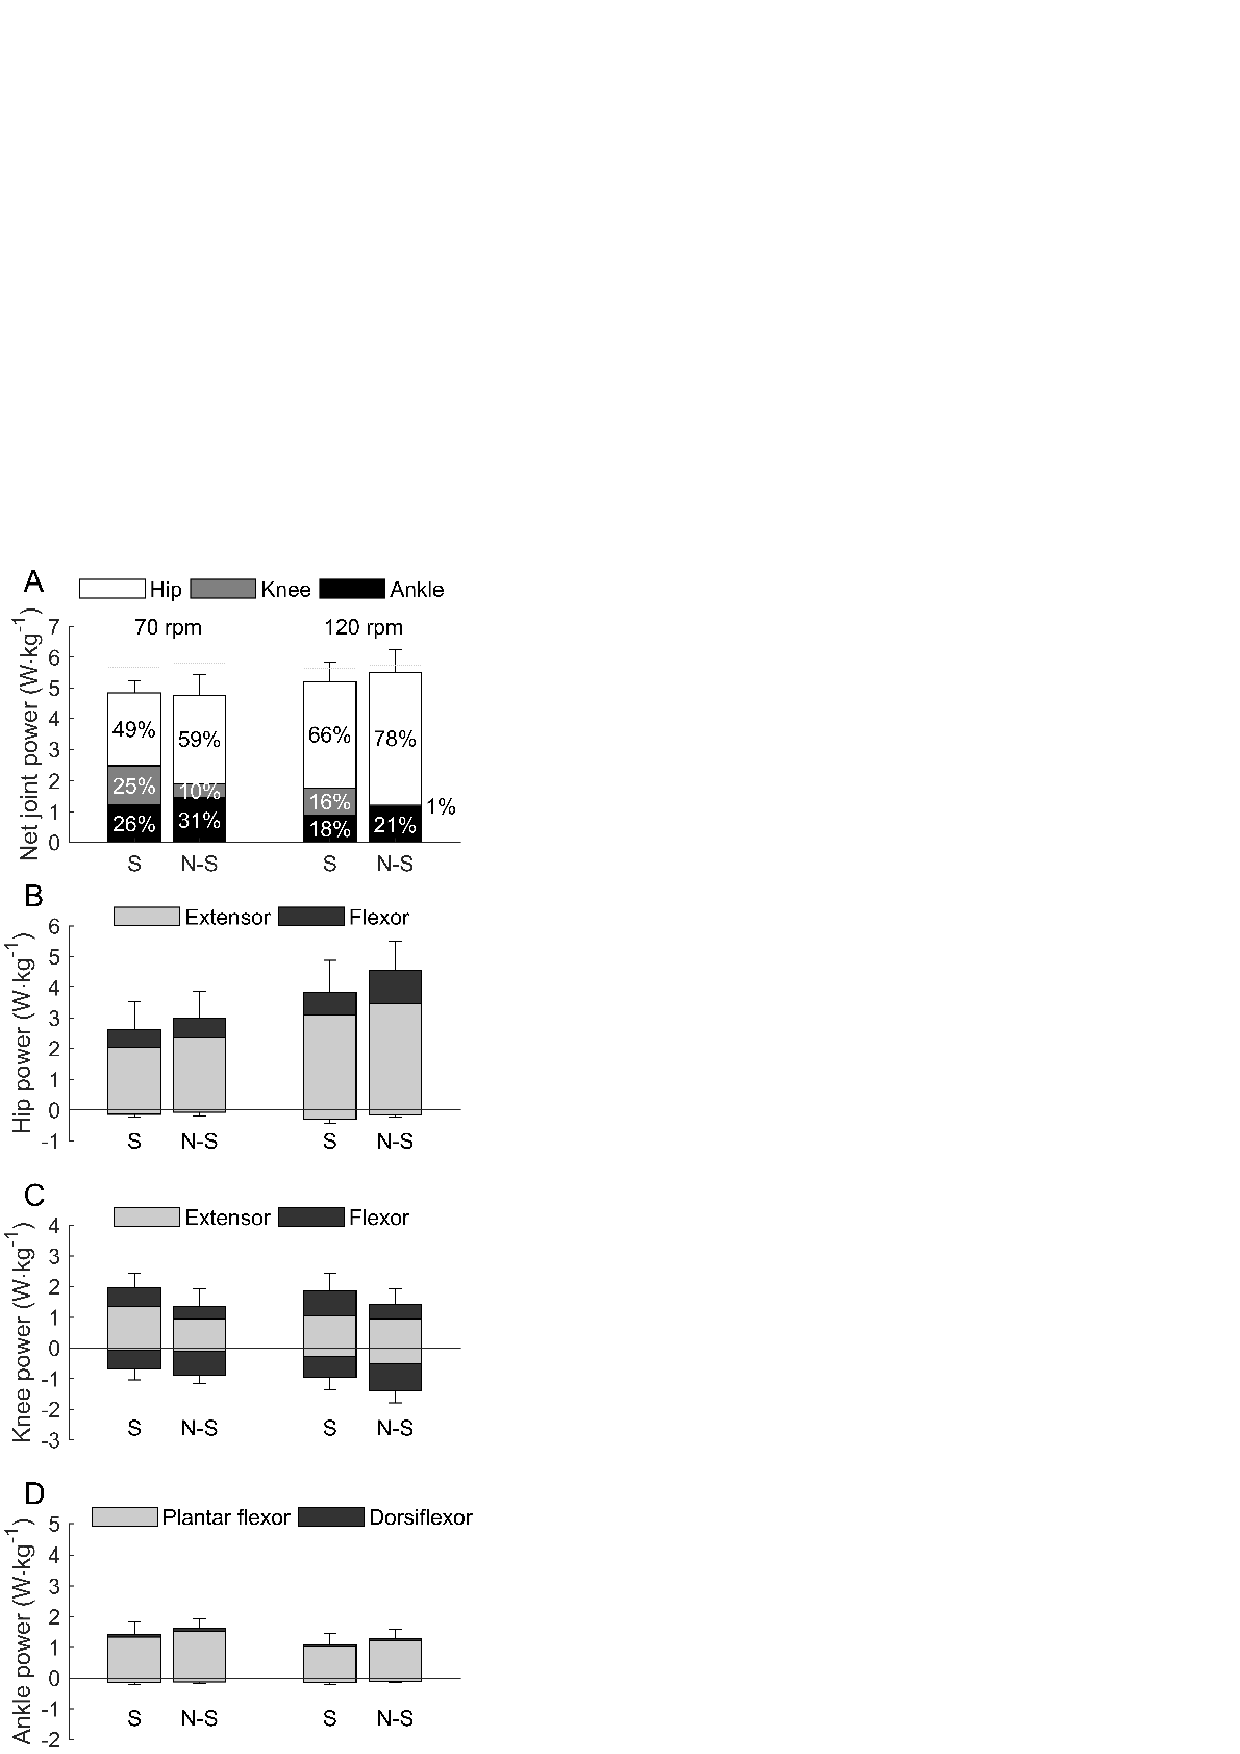
\includegraphics[width=0.48\textwidth]{Study1/Figure3.png}
    \caption[The net mechanical power contribution at the knee was significantly reduced by switching to a non-seated posture. ]{\textbf{The net mechanical power contribution at the knee was significantly reduced by switching to a non-seated posture.} A. Total lower limb joint power (mean $\pm$ SD) per cycle during seated (S) and non-seated (N-S) cycling at $70$ rpm and $120$ rpm. Stacked bars show the net power contribution ($\%$) at the hip, knee and ankle to total lower limb power. The breakdown of joint power into positive and negative contributions during net flexor and extensor muscle moments is shown for the hip (B), knee (C) and ankle (dorsiflexor/ plantar flexor) (D). n.b.: The reduction in net knee power is the result of large amounts of positive and negative power at the knee.}
    \label{fig:m1f3}
\end{figure}

\FloatBarrier

An unsurprising, but noteworthy result was the discrepancy in power between the ergometer, cranks, and lower limb. Power measured at the crank was marginally greater than power measured by the ergometer which was likely due to power losses in the drivetrain. Lower limb power was significantly lower than crank power in all conditions except for when in the non-seated posture at 120 rpm, likely due to contributions of the upper body to crank power. At 70 rpm, lower limb power accounted for 82 $\pm$ 5$\%$ of crank power when non-seated and 86 $\pm$ 5$\%$ when seated. At 120 rpm, lower limb power accounted for 96 $\pm$ 9$\%$ when non-seated and 92 $\pm$ 6$\%$ when seated. Previous research \autocite{Turpin2016} has shown that muscle activity within the upper limbs and handlebar forces increase significantly during high power output cycling. Thus, it seems plausible that greater contributions of power from the upper body and upper limbs occur when higher crank force is required, especially when in the non-seated posture.

EMA at the knee was significantly greater when non-seated compared to seated at the time of peak resultant force production (F=103, p$<$.001, $\eta^2_G$=0.27) (Figure \ref{fig:m1f4}). The moderate interaction effect between posture and cadence (F=9.4, p=.008, $\eta^2_G$=0.1) meant that the increase in EMA at the knee when non-seated was greater at 70 rpm (S=0.34$\pm$0.09 vs. Non-S=0.52$\pm$0.15, t=6.1, p$<$.001, 95$\%$CI [0.1-0.3], ES=1.4) than at 120 rpm (S=0.29$\pm$0.07 vs. Non-S=0.35$\pm$0.08, t=3.5, p=.004, 95$\%$CI [0.02-0.1], ES=0.7). In both postures, there was a moderate increase in EMA at the hip (F=8.9, p=.01, $\eta^2_G$=0.08) and a small decrease in EMA at the ankle (F=17, p=.001, $\eta^2_G$=0.04) at 70 rpm compared to 120 rpm.

BF was the only muscle to show a main effect of posture on mean EMG RMS (Figure \ref{fig:m1f5}). At both cadences, there was a large decrease in BF activity in the non-seated compared to seated posture (F=92, p$<$.001, $\eta^2_G$=0.6). Predictably the mean EMG RMS signal of all muscles was higher at 70 rpm than at 120 rpm (p$<$.001) due to the increase in torque required to maintain the set power output, which was likely to be closer to a quasi-maximal power output for each participant at the cadence of 70 rpm \autocite{Gardner2007,Dorel2005}.

\begin{figure}
    \centering
    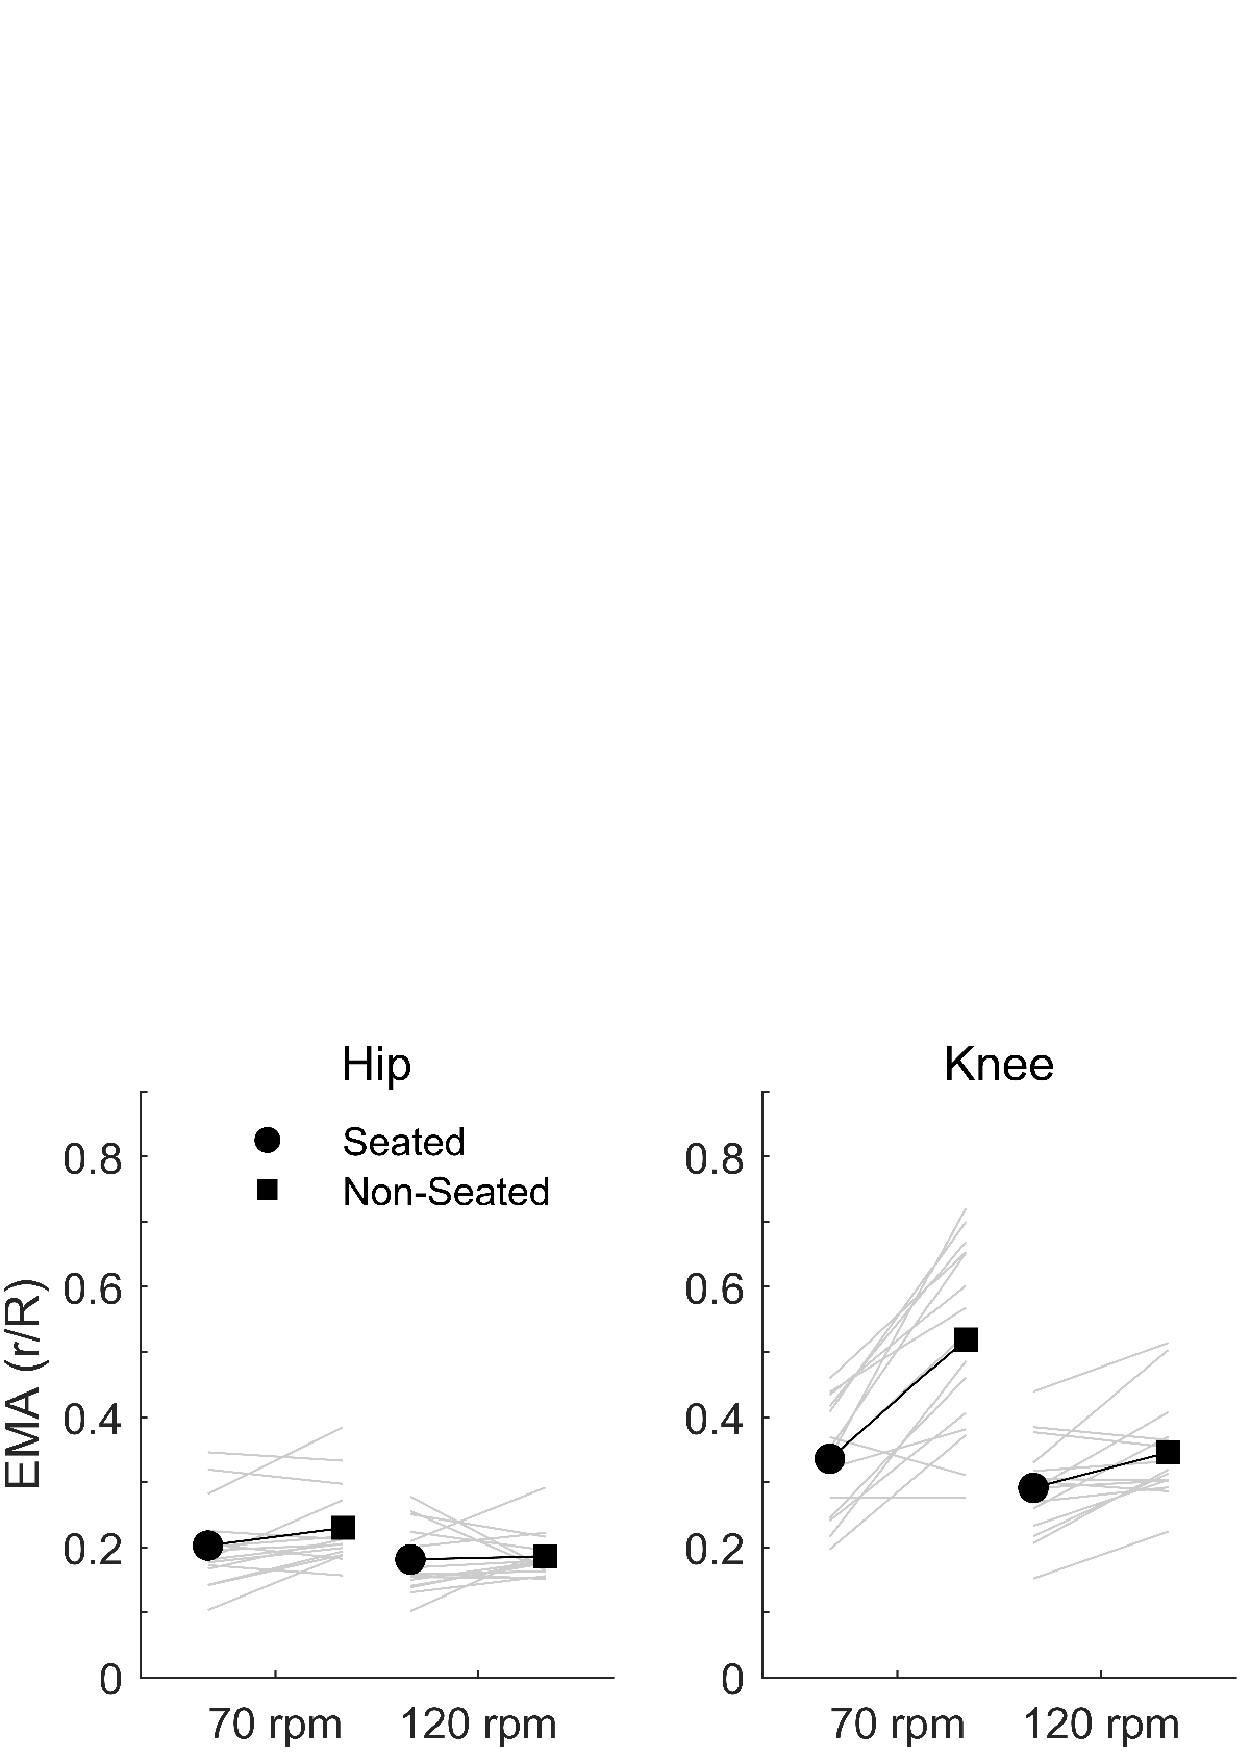
\includegraphics[width=\textwidth]{Study1/Figure4.png}
    \caption[Effective mechanical advantage at the knee was significantly increased by cycling in a non-seated posture at 70 rpm, but not 120 rpm.]{\textbf{Effective mechanical advantage (EMA) at the knee was significantly increased by cycling in a non-seated posture at 70 rpm, but not 120 rpm.} EMA of the hip, knee and ankle at the time of peak resultant crank force production in the seated (S) and non-seated (N-S) posture at 70 rpm and 120 rpm. Data for each participant (grey lines) is shown along with the group mean (black lines).}
    \label{fig:m1f4}
\end{figure}

\begin{figure}
    \centering
    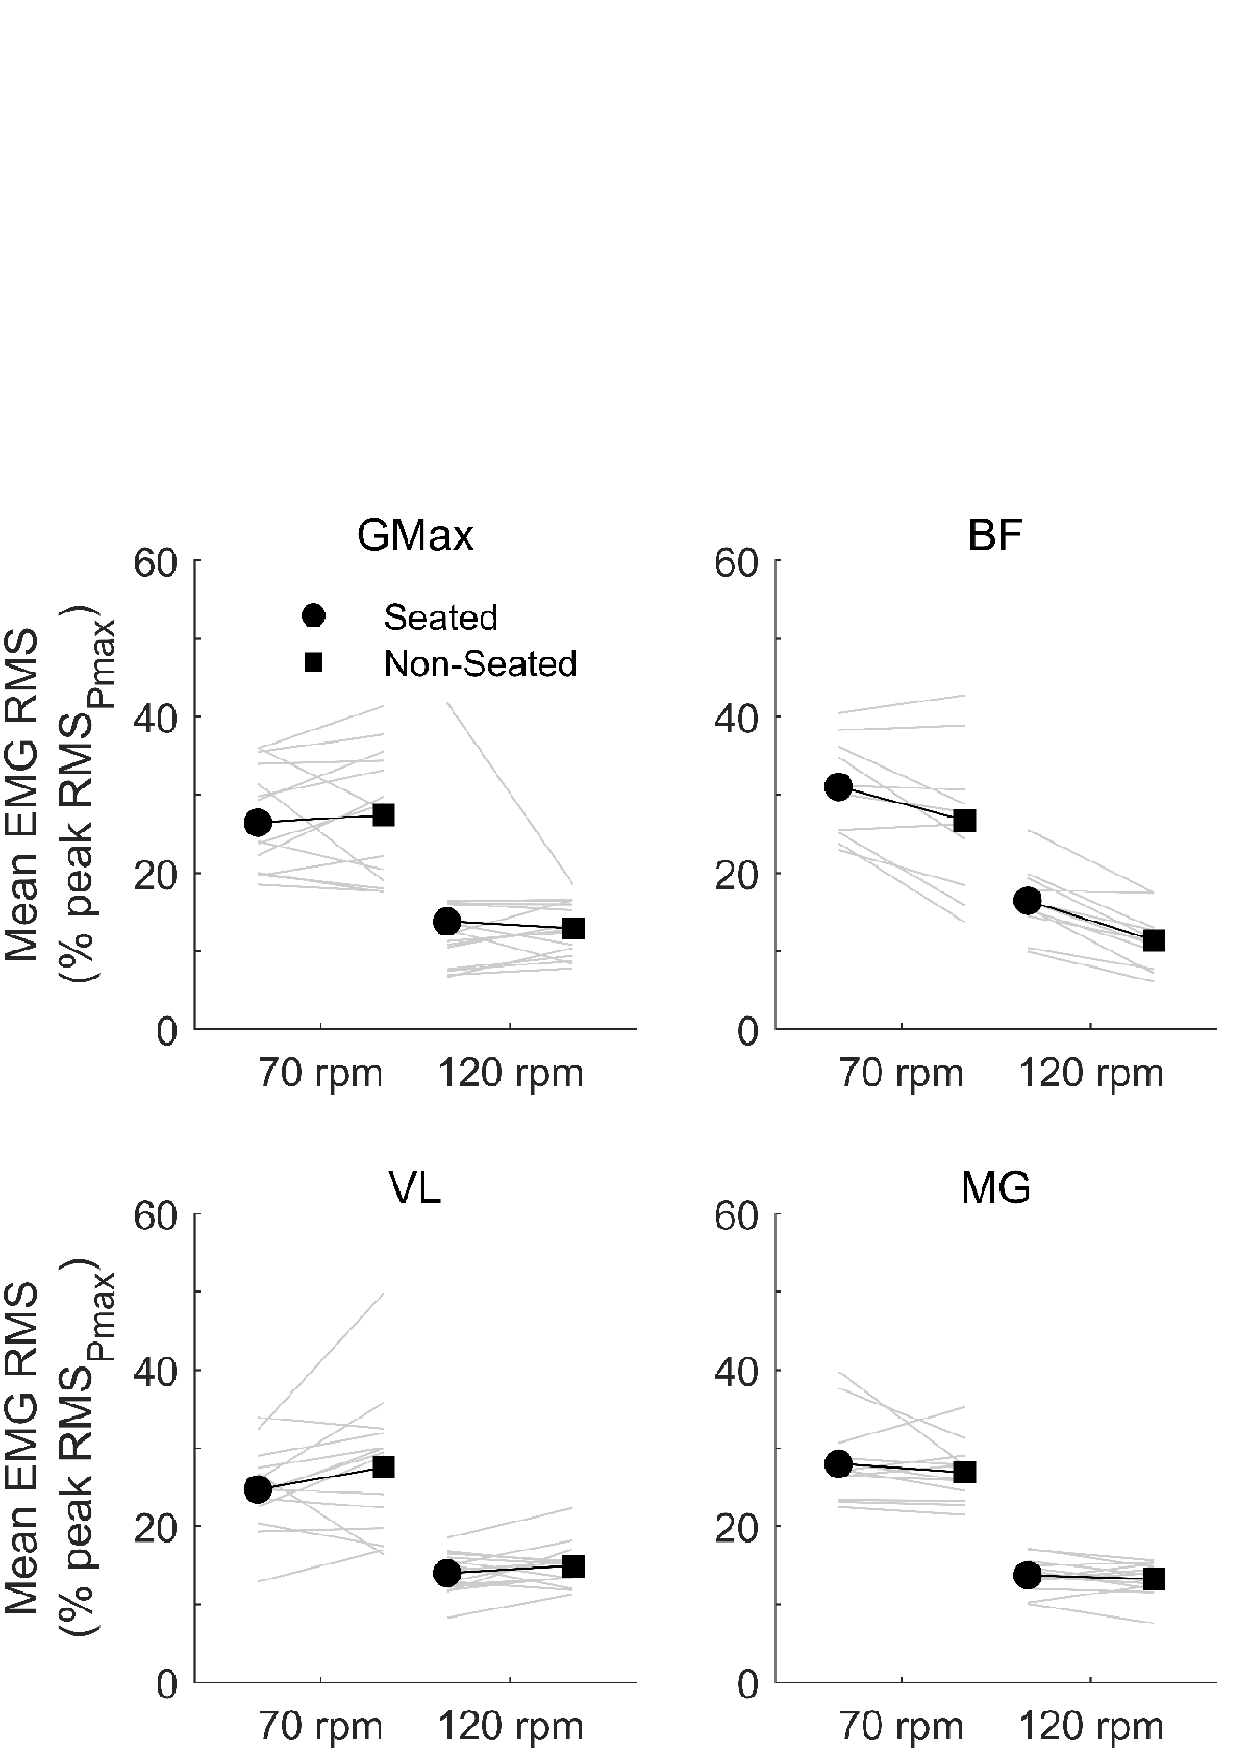
\includegraphics[width=\textwidth]{Study1/Figure5.png}
    \caption[Bi-articular hamstring activity was significantly reduced by cycling in a non-seated posture.]{\textbf{Bi-articular hamstring activity was significantly reduced by cycling in a non-seated posture.} Mean muscle activity (EMG RMS across the crank cycle, normalised to each muscle's peak RMS activity during the maximal sprint trial) for the gluteus maximus (GMax), rectus femoris (RF), biceps femoris (BF), vastus lateralis (VL), medial gastrocnemius (MG) and soleus (SOL) in seated (S) and non-seated (N-S) cycling at 70 rpm and 120 rpm. n.b.: Due to the increase in torque required per crank cycle, muscle activity was significantly greater at 70 rpm and 120 rpm for all muscles. Data for each participant (grey lines) is shown along with the group mean (black lines).}
    \label{fig:m1f5}
\end{figure}
\FloatBarrier

Statistical analysis was also performed on the magnitude and timing of peak joint angles, velocities and moments (See Table, Appendix \ref{tab:m1sdc2}, which summarises the significant main and interaction effects of posture and cadence). Of note is the 0.33 Nm$\cdot$kg$^{-1}$ reduction in the peak knee extension moment when non-seated at 70 rpm and the significant increase in peak knee extension angle when non-seated at 70 rpm (9$^\circ$) and 120 rpm (12$^\circ$) compared to when seated. Angular displacement, velocity and moments at the hip, knee and ankle with respect to crank angle have also been provided (See Figures, Appendix \ref{fig:m1sdc3}, \ref{fig:m1sdc4}, and \ref{fig:m1sdc5}) as well as EMG RMS signals with respect to crank angle (See Figure, Appendix \ref{fig:m1sdc6}).

\FloatBarrier
\section{Discussion}
The aim of this experiment was to compare power production across the hip, knee, and ankle between seated and non-seated cycling postures. This comparison was made when cycling at a very-high-power output (above the reported seated to non-seated threshold) at two different cadences (70 rpm and 120 rpm). The results support our primary hypothesis that joint power would be distributed away from the knee joint when cycling in a non-seated posture compared to when seated. In partial support of our second hypothesis, the redistribution of knee power due to the change in posture was different at each cadence, however, it was not re-distributed solely to the hip and ankle as we predicted. Cycling in a non-seated posture at 70 rpm resulted in 14$\%$ of crank power being re-distributed away from the knee to the hip (+8$\%$) and ankle (+4$\%$) compared to when seated. Cycling in a non-seated posture at 120 rpm resulted in 15$\%$ of crank power being re-distributed away from the knee to the hip (+13$\%$) and ankle (+4$\%$) compared to when seated. The discrepancy between the change in knee power relative to the summed change in hip and ankle power suggests there was a net gain in upper body power when cycling in a non-seated compared to seated posture at 70 rpm and a net loss in upper body power when cycling in a non-seated posture at 120 rpm compared to when seated. Cycling in a non-seated posture at 70 rpm also appears to increase the effectiveness of ankle power production, as higher levels of ankle power were produced without an increase in plantar flexor (MG, SOL) activity. At 120 rpm, hip power increased using similar levels of muscle activation in GMax and RF as at 70 rpm, but with lower levels of activation in BF, which may indicate that cyclists are more effective at producing hip power when in the non-seated posture. 

A key result of this study was that the non-seated posture increased negative power at the knee, which resulted in decreased net power at the knee. The increase in negative knee power, while the knee was extending, provides evidence that greater amounts of knee extension power are transferred away from the knee joint when non-seated. It is well understood that the coordinated activity of mono- and bi-articular muscles can serve to transfer energy across joints and orient the crank reaction force during the downstroke \autocite{Dorel2018b}. In light of this, it is important to note the individual muscle-joint designs of BF and MG \autocite{Lieber2011,Kuo2001}. For example, BF's moment arm is larger at the hip than at the knee, which means that co-contraction of VL and BF can transfer knee extension power to the hip. MG's moment arm is larger at the ankle than at the knee, which means co-contraction of VL and MG can transfer knee extension power to the ankle. Thus, shifting to a non-seated posture appears to utilise the ability of BF and MG to transfer knee extension power to the hip and ankle, respectively. 

In line with previous research \autocite{Caldwell1999}, joint moments at the hip, knee and ankle were significantly altered by the change in posture which suggests that transitioning to the non-seated posture when high crank forces are required can provide significant mechanical benefits. When non-seated at 70 rpm, peak extension moments at the hip, knee and ankle contributed to the resultant crank force being more closely aligned to the knee joint centre. As such, EMA at the knee was 53$\%$ higher in the non-seated posture (0.52 $\pm$ 0.15) compared to when seated (0.34 $\pm$ 0.09) at 70 rpm. Net torque requirements at the knee were reduced when non-seated, however mean RMS activity of the knee extensors (VL, RF) was similar between postures. Given the cautious assumption that the measured EMG in VL and RF provides an indication of the active muscle volume within the knee extensors \autocite{Enoka2008}, it appears that when in the non-seated posture, riders were able to support their bodyweight while also fulfilling the external power requirement at the cranks using a similar active volume of knee extensor muscle.

It may also be the case that switching to a non-seated posture at 70 rpm increases the force producing capability of knee extensor muscles. The peak knee extension angle and range of motion increased significantly in the non-seated posture, however, the increased range of motion did not lead to an increase in the mean extension velocity. This is because a greater portion of the crank cycle was spent extending the knee. For example, when non-seated at 70 rpm, the period of knee extension was so great (59$\%$) that the mean knee extension velocity was actually 5.8$\%$ lower than when seated. As supported by the findings of Brennan et al. \autocite{Brennan2018}, the reduction in mean knee extension velocity in the non-seated (181 deg$\cdot$s$^{-1}$) compared to seated (192 deg$\cdot$s$^{-1}$) posture at 70 rpm would bring the fascicle shortening velocity of VL closer to its optimum for both efficiency and force production. Thus, it appears that rider's use extra degrees of freedom afforded in the non-seated posture to increase the force producing capabilities of knee extensor muscles. 

Power generated during hip flexion and knee flexion played a critical role in the differences in positive hip and knee power between postures. Interestingly, when in the non-seated posture at 120 rpm almost half of the 12$\%$ increase in the contribution of positive hip power was due to hip flexion power. We only measured the activity of one hip flexor muscle (RF) making it difficult to provide insight into this finding as other hip flexor muscles such as iliacus, psoas, and sartorius were likely responsible for this increase. At both cadences, a large portion of the 15$\%$ increase in positive knee power when seated compared to non-seated was due to knee flexion power. The increase in knee flexion power was not reflected by any difference in BF activity during the period of knee flexion power production between postures. Thus, the most likely explanation is other knee flexor muscles were responsible for this increase. Another explanation is the greater mean knee flexion angle when seated compared to non-seated may have shifted the fascicle operating lengths of the knee flexors closer to optimal and hence been more favourable for generating power \autocite{Brennan2018}. On the whole, it appears there is a greater reliance on knee flexors to contribute power when seated, while there is a greater reliance on hip flexors to produce power when non-seated at 120 rpm. 

The limitations inherent to inverse dynamics \autocite{Zelik2012,Hicks2015} and quantifying surface EMG \autocite{Enoka2008} must be acknowledged when attempting to understand function and performance from an energetic perspective. One must consider that individual muscle force and power contributions cannot be inferred from joint-level analyses, nor can the level of neural drive to muscle be fully inferred from surface EMG. A further limitation pertains to the questionable ecological validity of ergometer cycling due to the constraint of frontal plane bicycle dynamics \autocite{Meijaard2007}. It has been shown that when bicycling in a non-seated posture in the field, cyclists sway the bike laterally underneath their body \autocite{Soden1978}, which might impact the power generating profile of different joints. Finally, accurate conclusions were unable to be made about which technique would be more economical, as metabolic cost (oxygen consumption) was not measured. However, due to the high power output and short duration of the conditions tested here, it is unlikely that the rate of metabolic energy expenditure with respect to time or per unit distance was the variable being optimised in either posture.

In summary, the contribution of knee joint power to total leg power was reduced by switching from a seated to non-seated posture during very-high-power output cycling. The decrease in net knee power when in the non-seated posture is likely the result of power produced by knee extensors being transferred by bi-articular muscles to the hip and ankle. This coordination strategy and increase in EMA at the knee joint means it is likely that both non-muscular and muscular power is more effectively transferred to the crank compared to when seated. These results highlight important differences in joint power contributions during seated and non-seated cycling, which may be a fundamental aspect of why cyclists choose to frequently use a non-seated posture when needing to produce very-high levels of crank torque and power.